\startfirstchapter{Introduction}
\label{chapter:introduction}



\section{The Localization Problem} \label{problem}

Geolocation is a rapidly growing field due to the large impact it has on daily life, the general public has become increasingly dependent on it for real-time navigation, particularly on mobile smartphone devices. Location-based services are  playing an increasingly important role in other fields such as teleconferencing, wireless communications, surveillance, and geophysics \cite{Cheung, classMDS, CheungChan, Huang, LiHu,  Sayed,
ShcauRob, SmithAbel,  Yao}.

Different technologies have been used to build geolocation systems. Several global navigation satellite systems that are available for both military and civilian use include GPS(US), Galileo(EU), GLONASS(Russia), BeiDou(China). Satellites are equipped with atomic clocks that provide a high-accuracy timing signal to  allow a receiver to calculate the time that it takes the signal to reach the receiver. This information is used to calculate the position of the receiver by using a  computational technique known as trilateration. The location of the receiver can be calculated from the
tracked positions of the satellites and the times measured, each known as the Time-of-Arrival (TOA) \cite{GeoLoc}.
%Consequently, it
%has been incorporated into many services and applications. Currently, outdoor
%localization, thanks to GPS, has revolutionized navigation-based applications running on automotive GPS-enabled devices and smart phones. Applications range from location awareness, to point-by-point directions between destinations, to identifying the closest cinema or coffee shop. The success of GPS has been due to the reliability, availability, and practical accuracy that the system can deliver; however, GPS lacks coverage indoors and in urban areas, in particular near buildings when the signal is blocked;
%even in the best of conditions, the accuracy is on the order of several meters. 
%navigation:
%auto
%aerial
%ships and boats
%heavy equipment
%fitness trackers (for example, Garmin gps enabled smart watches for tracking the run distance/routes/speed)
%
 GPS is widely used in navigation of vehicles such as airplanes, ships, and heavy equipment. It has also been used for monitoring movements rather than navigating, for example in fitness trackers such as FitBit \cite{FB} and Garmin\cite{Garmin} which automatically collect data about the user's activities (distance run, speed, routes taken).
 

As location-based services are becoming increasingly integrated into daily life,  the demand for more accurate and robust localization technologies, including in GPS-denied areas, has increased. One of the approaches to the problem was integration of various wireless technologies with GPS. One such solution is called Assisted GPS (A-GPS), which distributes data and processing over a network of cellular towers equipped with GPS-enabled servers \cite{AGPS}. This can greatly reduce the search space and time to first fix on location. Other systems were built purely on cellular signals, adapting the TOA techniques originally developed for GPS. However their accuracy was limited in urban environments due to obstruction of signals by buildings, and the technique did not gain widespread use beyond the Emergency-911 system it was developed for in the United States.

% Paper: http://www.cs.columbia.edu/~drexel/CandExam/Geolocation_assistedGPS.pdf

With the proliferation of smartphone devices and the internet, WiFi access points are becoming increasingly widespread, providing another means of determining location. One type of WiFi-based technique is called Received Signal Strength (RSS) location fingerprinting. It uses a database of WiFi signatures (RSS values and MAC addresses) with associated GPS coordinates. This has to be built up ahead of time, for example by surveying a city with a GPS and WiFi enabled vehicle. 
Real-time location of the mobile device is determined using the pattern-matching technique, that compares the measured RSSs between the mobile device and access points, and the RSS values stored in the database. Skyhook Wireless successfully developed such system that delivers accuracy of tens of meters in urban areas \cite{Skyhook}. 

Design of any localization system naturally includes a trade-off between the overall performance and cost requirements. Some of the systems developed so far take advantage from the knowledge of the surrounding infrastructure such as
cell towers, Wi-Fi hot spots, or installed RF tags \cite{GeoLoc}. Usually, the precision of the localization in such systems depends on the infrastructure. For example,  hundreds or thousands of meters for cellular survey-based techniques, tens to hundreds of meters, or less than 100 meters for cellular triangulation techniques.

%\textbf{indoor loc - 1 paragraph}

Indoor environments have additional challenges such as limited coverage, multipath signal fading and NLOS conditions. At the same time, indoor applications typically require greater accuracy due to the smaller spaces involved. Robotics was one early application area \cite{Durant}. Systems such as CISCO Wireless Location Application \cite{CiscoWLA} have applied RSS fingerprinting to indoor positioning, which works well if it is acceptable to install the required infrastructure and only coarse positioning is required. In searching for a method that would provide higher accuracy and be more robust in NLOS conditions, researches shifted their focus to Ultra-Wideband (UWB) communications which allow much more accurate timing information to be obtained. Another advantage of UWB is that it has increased bandwidth and helps prevent multipath signal fading \cite{AlaviUWB}.

Combining sensor data from multiple sources to improve localization results is another active area of research. Simultaneous Localization and Mapping (SLAM) is one such technique. The algorithm generates a map of the environment using RF signal, inertial sensors, images, Light Detection and Ranging (LIDAR) and sonar. A topological map is produced which can be used for navigation.



\section{Basic Localization Systems}

Many different systems have been developed for solving the localization problem in different domains such as geolocation, indoor positioning, sonar, etc. Despite the fact that the  solutions themselves are different, they share some fundamental concepts. Classical non-survey based localization systems  are generally comprised of two subsystems: range/angle estimation subsystem and lateration/angulation subsystem \cite{GeoLoc}. The range/angle estimation subsystem determines distance or direction between the  mobile object of unknown location  and an array of reference points with known location  either pre-programmed or obtained through GPS.  The reference points can be satellites in GPS technology, or base stations in cellular localization, or a set of iBeacons, etc. Lateration/angulation subsystem uses the coordinates of the reference points and the distance or angle estimates to determine the unknown position.  The accuracy of the positioning depends on the accuracy of the anchor nodes’ position, the quality of the range/angle estimates, network geometry, and the performance of the localization algorithm. Figure \ref{fig:2step} illustrates this two-step procedure.


\begin{figure*}[h]
\centering
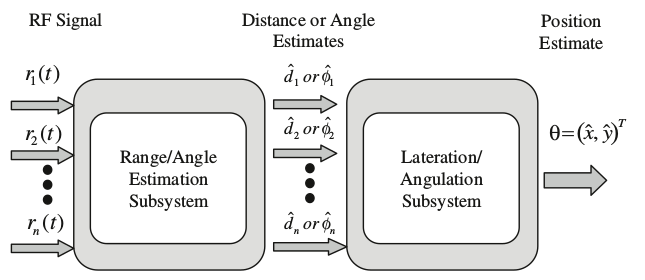
\includegraphics[width=1.0\textwidth]{figures/localization_example.png}
\caption{Classical geolocation system. Range or angle information is extracted from received RF signals. Location is then estimated by lateration/angulation techniques \cite{GeoLoc}.}
\label{fig:2step}
\end{figure*}


In the rest of this section, we  provide an overview of the most popular ranging localization methods, namely  TOA, TDOA, AOA, and RSS.



\subsection{Time of Arrival Method}

Time of Arrival (TOA) localization is a part of class of range-based localization techniques and is often referred to as tri-lateration. It uses the fact that knowing the propagation speed of  signals between a mobile device and reference points and by measuring the time that a signal takes to be received, the distance can easily be calculated. To obtain an $n$  dimensional position estimate at least $n+1$ range measurements are required. Note that absolute times are used in calculations, so it is critical that the  clocks in base stations and the mobile device are synchronized. It is also assumed that they are all in LOS condition. %Unfortunately, this is not always the case in practice. %In many situation this is not practicle.

Solution techniques developed for range-based localization can be categorized as Maximum Likelihood (ML) and Least Squares (LS) approaches. 
Given the observed range measurements $\Br_n = \Br + \Bw$, the ML estimate $\hat{\Bx}$ of the unknown source location $\Bx$ is obtained by maximizing the conditional probability density function 
\begin{equation}
\nonumber
\hat{\Bx} = \mbox{arg}\max_{\Bx} P\left(\Br_n|\Bx\right)
\end{equation}
where $\Bw$ represents measurement noise. One of the major problems with ML approach is that it requires the knowledge of exact error-free measurements. Another difficulty is that solving for the unknown position estimate is computationally difficult. Many variants and approximations of the original ML has been  developed \cite{HoML}, \cite{Guvenc2}, \cite{Guvenc}.

In LS approaches, the source location estimate $\hat{\Bx}$ is found by minimizing the sum of residuals \cite{GeoLoc}
\begin{equation}
\nonumber
\hat{\Bx} = \mbox{arg}\min_{\Bx} \left\lbrace \sum_{i=1}^m \beta_i\left(r_n^{(i)} - \|\Bx - \Ba_i\|\right)^2 \right\rbrace
\end{equation}
where $\Ba_i$ is a vector of known coordinates of reference points (sensors),   $r_n^{(i)}$ is a noisy range measurement associated with it, $\beta_i$ is a weight
that can be used to emphasize  the degree of confidence in the measurement, and $m$ is the number of sensors. This problem is hard to solve in general because it is a nonconvex problem. Detailed analysis and discussion on solution methods for this problem will be given in Chapters 2, 3, and 4.


\subsection{Time Difference of Arrival Method}

A TDOA system is comprised of at least three base stations, one of which is the reference station. All stations are transmitting at precise time intervals, and the receiver measures the small differences in time that it takes the signals to arrive. From this information it is able to calculate its position. 
An important property of TDOA is that it requires base stations to be synchronized with each other, but it does not require the mobile receiver to be synchronized with the base stations. This technique first found application
%First TDOA, also known as hyperbolic, localization techniques emerged in the field of geolocation 
in 1940s, when it was used by the British Royal Air Force for guiding airplanes at night. At that time synchronization between measuring stations was not possible. Therefore TDOA techniques were feasible, while TOA were not. TDOA remains an important technique, finding modern application in 3G and LTE networks \cite{Ascom}.

% Using the time diff. for example, first geolocation systems for acoustic localization in 40 - to shoot ships.
%The basic idea is that 

The conventional TDOA-based localization technique is a problem of solving a set of hyperbolic equations. More details can be found in Secs. 2.2 and 4.1 of the thesis.

\subsection{Angle of Arrival Method}

In the case of Angle of Arrival localization, the base stations are able to measure the angle of signal arrival with respect to an absolute reference. 
Knowing the location of base stations, the user position can be calculated as an intersection point of two lines that pass through the base stations \cite{Dempster}
\begin{equation}
\nonumber
\Bx = \begin{bmatrix}
tan\phi_1 & -1 \\
tan\phi_2 & -1
\end{bmatrix}^{-1} \begin{bmatrix}
x_1 tan\phi_1 & -y_1 \\
x_2 tan\phi_2 & -y_2
\end{bmatrix}
\end{equation}
Figure \ref{fig:aoa} depicts the geometric principle of AOA technique. Even though AOA localization is relatively simple, it did not gain widespread usage because of poor performance in severe NLOS multipath scenarios. However, AOA has been used in hybrid positioning techniques along with TOA providing better performance than individual systems \cite{ChangChang}.  


\begin{figure*}[h]
\centering
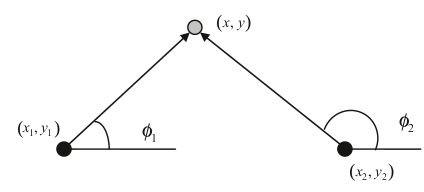
\includegraphics[width=0.7\textwidth]{figures/angle_of_arrival.png}
\caption{AOA positioning (angulation). The AOA estimate from 2 base stations to the mobile terminal can be used to estimate the position \cite{GeoLoc}.}
\label{fig:aoa}
\end{figure*}


\subsection{Methods Based on Received Signal Strength}

The localization technique based on received signal strength is very similar to the TOA method in the sense that the estimate of the unknown position of the mobile device/radiating source is obtained from the range distance measurements between the sensors and the object.
The difference is in the way a range measurement itself is obtained. In TOA method the range is obtained from the time reading through scaling, whereas in the RSS method the range is obtained from the received signal strength. 
The main idea that justifies this type of localization is that the strength of the RF signal attenuates with distance. The relationship between the RSS reading and the distance can be approximated by a log-normal attenuation model \cite{LiuSurvey}
\begin{equation}
\nonumber
P_x(d) = P_0(d_0) - 10n_p\log_{10}\left(\frac{d_i}{d_0}\right) + X_{\sigma}
\end{equation}
where $P_0(d_0)$ is a reference power in dB milliwatts at a reference distance $d_0$ away from the transmitter, $n_p$ is the pathloss exponent governing the rate of power decay with distance, $X_{\sigma}$ is the log-normal shadow fading component, and $d_i$ is the distance between the mobile devices and the $i$th base station. Both $\sigma$ and $n_p$ are environment dependent. Given the model and model parameters, which are obtained via a priori measurements, the inter-sensor distances can be estimated from the RSS measurements. Localization algorithms can then be applied to these distance measurements to obtain estimated locations of sensors.

\section{Contributions and Organization of the Thesis}

\subsection{Contributions  of the Thesis} \label{contributions}

%the material developed here / mathematical tools and methods are suitable for many different scenarios 
%OR
%can have different world life applications, for example: TOA, TDOA, static positioning using UWB range measurements. 

This thesis investigates new solution methods for single source localization problems that are potentially applicable to wireless sensor networks where range or range-difference measurements can be obtained utilizing RF signals. We remark
that the methods and solution techniques proposed in the thesis are of general nature, and hence potentially useful in other scenarios that include localization problems for networks involving  ultrasonic, sonic, or light sensors. 
In this thesis we focus on the least squares approaches for estimating the source location. Our models assume the availability of range or range-difference measurements and do not take into account the nonline-of-sight (NLOS) scenarios. Such simplifying assumptions are often made \cite{Cheung}, \cite{classMDS} since mitigating the NLOS conditions is a separate research area. The main challenge facing the thesis research is that the localization problems we investigate
are nonconvex problems whose global solutions are difficult to identify, although many
approximate solutions \cite{Cheung}, \cite{LiHu},  \cite{SmithAbel}, and data fusion methods \cite{Sayed} have been developed. The main contributions of the thesis can be summarized as follows:

\begin{itemize}
\item
Development of an iterative re-weighting algorithm for range-based localization based on squared range-based least squares;

\item
Development of a iterative re-weighting algorithm for range-difference-based localization based on squared range-difference-based least squares;

\item
Development of a penalty convex-concave procedure (PCCP) for single source localization based on range measurements;

\item
Development of a sequential convex relaxation procedures for efficient computation of the LS estimate of source coordinates for range and range-difference localization.


\end{itemize}


\subsection{Organization of the Thesis} \label{organization}

The organization of the thesis is  as follows:

\phantom{m}

\noindent
\textbf{Chapter 1 - Introduction}

\phantom{m}

\noindent
The purpose of this chapter is to introduce the systems and methods developed for the localization problems, discuss the motivations for improving the existing methods, and describe the main contributions and structure of the thesis.


\phantom{m}

\noindent
\textbf{Chapter 2 - Iterative Re-Weighting Least-Squares Methods for Source Localization}


\phantom{m}

\noindent
This chapter presents improved least squares methods that are iterative in nature. At each iteration the algorithms find a global solution to a subproblem that, as iterations proceed, approximates closely the LS solution.


\phantom{m}

\noindent
\textbf{Chapter 3 - Penalty Convex-Concave Procedure for Source Localization}


\phantom{m}

\noindent
In this chapter an algorithm is developed for finding an approximate solution to nonlinear least squares problem, for the case of range-based localization. We focus on the least squares formulation for the localization problem, where the $l_2$-norm of the residual errors is minimized in a setting known as difference-of-convex-functions programming. The problem at hand is then solved by applying a penalty convex-concave procedure in a successive manner.


\phantom{m}

\noindent
\textbf{Chapter 4 - Least Squares Localization by Sequential Convex Relaxation}


\phantom{m}

\noindent
This chapter addresses localization of a single radiating source based on range or range-difference measurements. In both cases the focus is on efficient computation of the least squares estimates of the source coordinates. For the case of range-difference, the central part of the procedure is a convex quadratic programming problem that needs to be solved in each iteration to provide an increment vector that updates the present iterate to the next towards the solution of the localization problem at hand.

\phantom{m}

\noindent
\textbf{Chapter 5 - Conclusions}

\phantom{m}

\noindent
The chapter summarizes the main results achieved in the thesis and suggests several problems for future studies in the area.
